\documentclass[twoside,numberorder]{csbachelor}
%==============================================================
%==============================================================

\usepackage{url}
\usepackage{subfigure}
\usepackage{pdfpages}
\usepackage[numbers]{natbib}
\citestyle{IEEEtran}


%一些全局工具的定义
\DeclareMathOperator*{\argmin}{arg\,min}
\DeclareMathOperator*{\argmax}{arg\,max}

%==============================================================
%==============================================================
\begin{document}
%==============================================================
%==============================================================

  %论文题目:{中文}{英文}
%   \zjutitle{基于Dynamic Memory Network的问答系统的优化与应用}%
%            {}
%   %作者:{中文姓名}{英文}{学号}
%   \zjuauthor{杨凯}{Yang Kai}{3130000495}
%   %指导教师:{导师中文名}{导师英文名}
%   \zjumentor{蔡亮}{Cai Liang}
%   %个人信息:{年级}{专业名称}
%   \zjuinfo{2013级}{软件工程}
%   %学院信息:{学院中文}{学院英文}
%   \zjucollege{计算机科学与技术}{College of Computer Science and Technology}
%   %日期:{Submitted Date}
%   %\zjudate{2017年3月20日}

% %==============================================================

%   %封面
%   %%============================================================
%% 中文封面

\thispagestyle{empty}

\vspace{5mm}

\begin{center}
   
\includegraphics[width=108mm]{images/zjdx}
\end{center}

\centerline{\heiti\erhao\textbf{本科生毕业论文}}
\centerline{\heiti\erhao\textbf{开题报告}}
\vspace{4mm}

\begin{center}
  
\includegraphics[width=35mm]{images/standxb}
\end{center}

\vspace{25mm}

% {\hspace{16mm}\songti\sanhao\bfseries 题目:
%   \hspace{2mm} \begin{minipage}[t]{98mm}\linespread{1.1}\uline{\zjutitlec}\end{minipage}}

\vspace{7mm}

\begin{tabbing}
     \= \songti\sihao 题\hspace{10mm}目: \= \underline{\makebox[12cm]{\sihao\zjutitlec}} \\[2mm]
    \> \songti\sihao 姓\hspace{10mm}名: \= \underline{\makebox[12cm]{\sihao\zjuauthornamec}} \\[2mm]
    \> \songti\sihao 学\hspace{10mm}号: \> 
    \underline{\makebox[12cm]{\sihao\zjuauthorid}} \\[2mm]
    \> \songti\sihao 指导教师: \> \underline{\makebox[12cm]{\sihao\zjumentorc}} \\[2mm]
    \> \songti\sihao 专\hspace{10mm}业: \= \underline{\makebox[12cm]{\sihao\zjugrade\hspace{3mm}\zjumajor}} \\[2mm]
    \> \songti\sihao 学\hspace{10mm}院: \> \underline{\makebox[12cm]{\sihao\zjucollegec}}
\end{tabbing}


%%============================================================
% empty page for two-page print
\ifthenelse{\equal{\zjuside}{T}}{%
  \newpage\mbox{}%
  \thispagestyle{empty}}{}
%   %诚信承诺书
%   %% mentorassign

\newpage
\thispagestyle{empty}

\begin{tabbing}
\hspace{5mm}\songti\sihao 一、题目:\underline{\makebox[12cm]{基于Dynamic Memory Network的问答系统的设计与实现}}
\\ \\
\hspace{5mm}\songti\sihao 二、指导教师对开题报告、外文翻译和文献综述的具体要求:
\end{tabbing}
\begin{itemize}
\item 要求查阅相关的文献10篇以上(外文不少于5篇)。
\item 翻译的外文文献必须是研究性的论文,并且与论文主题直接相关.
\item 文献综述应包括国内外现状、研究方向、存在问题、参考依据等方面情况。
\item 译文和文献综述字数要求各3000字以上,开题报告字数为3500字以上。
\item 开题报告的内容应包括:
\begin{enumerate}
\item 主要研究内容、目的和意义;
\item 有关的国内外研究状况;
\item 课题难点和拟解决的关键问题;
\item 拟取的研究方法及其可行性、预期达到的目标;
\end{enumerate}
\end{itemize}
\vspace{60mm}

\begin{tabbing}
\hspace{80mm}\songti\xiaosi 指导教师(签名):
\\ \hspace{90mm} \songti\xiaosi 年 \hspace{5mm} \songti\xiaosi 月 \hspace{5mm} \songti\xiaosi 日
\end{tabbing}

\ifthenelse{\equal{\zjuside}{T}}{%
  \newpage\mbox{}%
  \thispagestyle{empty}}{}

%   %考核
%   %考核
\thispagestyle{empty}
{
\begin{center}
\stfangsong\sihao 毕业论文开题报告、外文翻译和文献综述考核
\end{center}
}
{\songti\sihao 导师对开题报告、外文翻译和文献综述评语及成绩评定:}
\\
\\  论文的文献综述部份对自然语言问答技术以及 Dynamic Memory Network的现状、研究方向等内容进行了分析,文献综述与论文的方向一致。开题报告对论文工作的主要内容、研究计划、预期进展等方面进行了相关介绍,外文翻译的术语翻译正确,符合要求,同意进入毕业设计的下一阶段。\\
\\
\\

{
\hspace{3cm} \songti\xiaosi
\begin{tabular}{|c|c|c|c|}
    \hline
    成绩比例 & \parbox[t]{4em}{开题报告\\[-1.5em]占(20\%)} &
               \parbox[t]{4em}{文献综述\\[-1.5em]占(10\%)} &
               \parbox[t]{4em}{外文翻译\\[-1.5em]占(10\%)} \\

    \hline
    分值   & & &  \\
    \hline
\end{tabular}
}
\begin{flushright}
    导师签字\;\underline{\hspace{4em}}\\
    年 \quad 月 \quad 日
\end{flushright}

{\songti\sihao 答辩小组对开题报告、外文翻译和文献综述评语及成绩评定:}
\vspace{4cm}

{
\hspace{3cm} \songti\xiaosi
\begin{tabular}{|c|c|c|c|}
    \hline
    成绩比例 & \parbox[t]{4em}{开题报告\\[-1.5em]占(20\%)} &
               \parbox[t]{4em}{文献综述\\[-1.5em]占(10\%)} &
               \parbox[t]{4em}{外文翻译\\[-1.5em]占(10\%)} \\

    \hline
    分值   & & &  \\
    \hline
\end{tabular}
}
\begin{flushright}
    答辩小组负责人(签名)\;\underline{\hspace{4em}}\\
    年 \quad 月 \quad 日
\end{flushright}



% %==============================================================
% %这部分不需要自己修改。

%   %目次页
%   \tableofcontents
%   \thispagestyle{empty}
%   \chaptermark{目录}
%   %\addcontentsline{toc}{chapter}{目录}

%   \mainmatter

% %==============================================================

%   %\chapter{本科毕业论文开题报告}
\setcounter{page}{1}
{\sanhao\heiti\filcenter \centerline{本科毕业论文开题报告}}
\section{课题背景}

人类语言具有特殊的结构,能够方便的传达意义,自然语言处理(NLP)就是研究人类语言的一个学科。而问答系统(Question Answering)的NLP问题之一。NLP中的很多问题都可以转换为QA问题(例如:机器翻译、情感分析、实体标记等)。随着智能语音助手(例如:苹果的Siri、谷歌的Google Assistant和微软的Cortana)的流行,
QA问题更是被广泛的予以关注。而QA问题本身是一项很复杂的NLP任务。想要对问题做出回答,需要具有分析一段文字,进行归纳总结的能力。\\
传统的解决QA的方法通常依赖于固定结构的知识数据库,而这些数据库通常是由特定领域的专家人工搭建的。当进行问题回答时,首先解析问题,然后将问题转换成特定结构的查询语句,在数据库中搜寻,在将查询结果组合成回答呈现给用户。\\
随着深度学习领域的迅速发展,以神经网络为基础的方法已经在文字和图像分类识别领域取得了重大的进展。最近,开始逐渐有人将神经网络应用于比较复杂的任务,例如逻辑推理上。这些通过神经网络产生的隐式的语言表达不需要依赖于特定的语言结构,
也不需要对语言做特定对解析等预处理行为。这些模型在需要很少的预处理过程的前提下,达到或者超过了传统的模型,取得了很好的结果。这些模型依赖于记忆(Memory)模块和注意力(Attention)模块,起到了能够从上下文总结信息、进行推理等作用。\\
Dynamic Memory Network就是这样一个使用了记忆和注意力模块的模型。这个模型在能够取得当前领先的结果。模型由四个模块组成:输入模块、片段记忆模块、问题模块、回答模块。\\
本毕业论文将给予Dynamic Memory Network,首先实现这一模型,然后再对这一模型进行进一步扩展优化,最后将我们优化后的模型应用于技术文档数据集中。\\
\section{目标和内容}
本次毕业论文主要任务是基于Dynamic Memory Network模型的优化及其应用,具体来讲,分为以下几个子目标:
\begin{itemize}
\item 实现基准模型,作为实验对照
\item 实现基础Dynamic Memory Network
\item 对Dynamic Memory Networt进行进一步优化(输入表达可以进一步尝试使用GloVe和基于字的词表达,记忆模块尝试使用GRU、LSTM和bidirectional LSTM优化)
\item 在单词回答的技术上支持多词回答
\item 将优化后的模型应用于技术文档数据集
\end{itemize} 
\section{可行性分析}
从下面几个角度分析,本次毕业论文是可行的:
\begin{itemize}
\item 实验模型:Kumar et al.\cite{DBLP:journals/corr/KumarISBEPOGS15}对这一基础模型的架构已经有了比较清晰的描述。使用主流的机器学习框架Keras和TensorFlow能够相应的减少一些所需要的基础工作量。
\item 数据集:使用Facebook bAbI数据集。数据集是公开可用的,已经被问答系统模型广泛使用和验证,有较为全面的基准可以用于实验的对比。
\item 实验机器:
    \begin{itemize}
    \item Macbook Pro 2016,16GB内存,2.60Hz Intel Core i7:代码编写,初步程序验证。
    \item Precision Tower 7810 Workstation,32GB内存,Intel Xeon i7, Nvidia GeForce GTX 970显卡:程序验证,高阶参数调整。
    \item Google Cloud Platform: 32GB内存,Nvidia Tesla K80显卡:训练数据。 
    \end{itemize}
\end{itemize}
\section{研究方案和关键技术考虑}
\subsection{研究方案}
本次实验采用对照实验,一个基准组和两个对照组。基准组是将词向量直接作为输入进入最简单的神经网络架构中,来实现的。一个实验组是实现Dynmaic Memory Network的基础模型的实验组,
另外一个实验组是对基础Dynamic Memory Network优化后的实验组。
本次实验使用Facebook bABi数据集。bABi数据集分成20个子集,每个子集具有不同的结构,图1.1为数据集中的一些例子\cite{DBLP:journals/corr/WestonBCM15}。每个子集有1000个训练样本和1000个测试样本。我们使用训练样本对我们的三个模型进行训练,
使用测试样本进行测试。一个模型只有能够正确回答95\%的测试集问题,则称之为能够通过这个子任务集。
\begin{figure}[h]
    \centering
    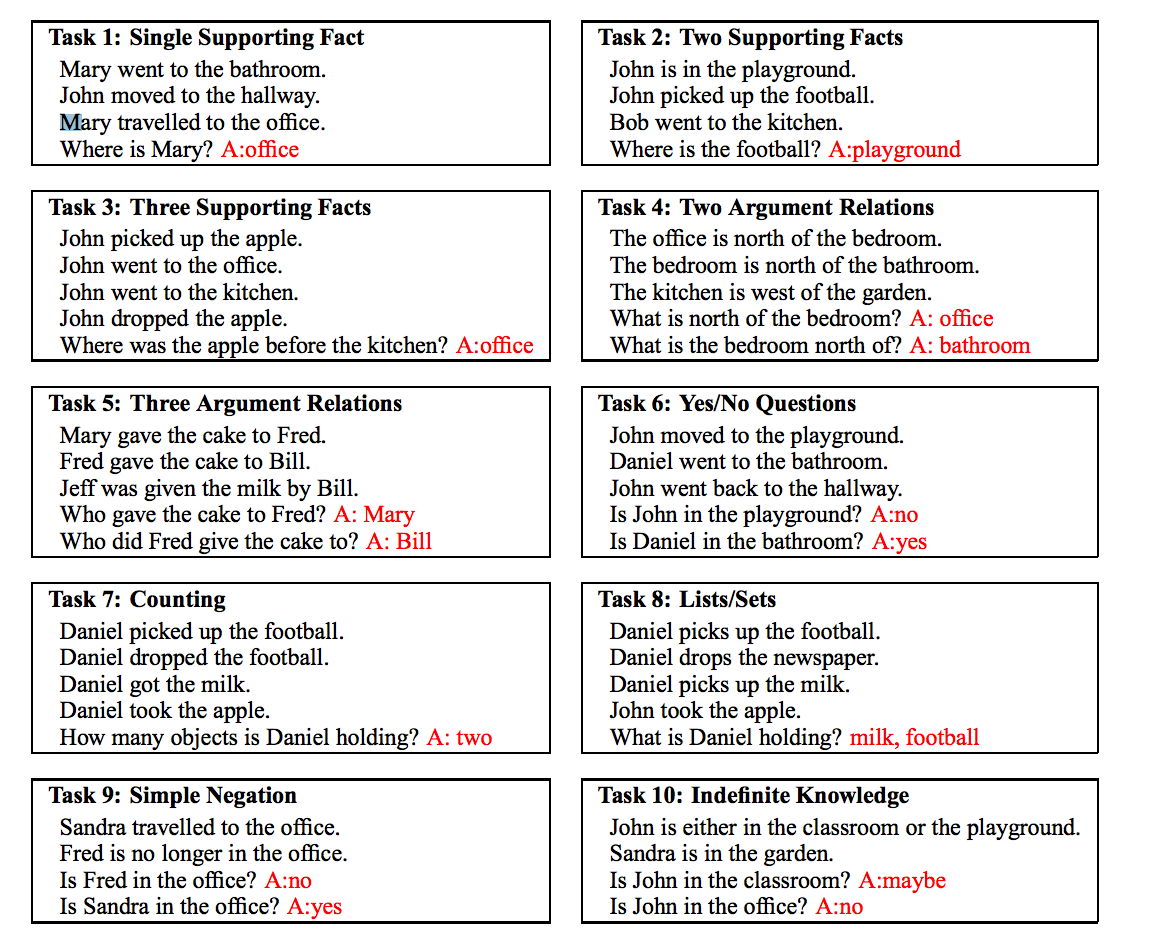
\includegraphics[width=0.6\textwidth]{./images/dataset-example}
      \caption{bABi数据样例}
    \end{figure} 
\subsection{Word2Vec}
Word2Vec(Mikolov et al., 2013\cite{mikolov2013efficient})是一种表达词汇的方法,将一个单词用一个向量来表示,关系比较近的词(例如:king和queen,Shanghai和Beijing)在向量空间相对应的有比较近的距离。如何确定词的关系,一个朴素的想法就是在相似上下文中出现的单词关系比较近。
Word2Vec就是基于这一想法的一种高效的词汇表达方法。特别的,Word2Vec有两种算法,分别是Continuous Bag-of-Words(CBOW)和Skip-Gram。CBOW是根据环境词预测中心词,而Skip-Gram是根据中心词预测环境词。\\
\subsection{GloVe}
尽管Word2Vec已经被实验证明可以发掘出复杂的语义相似关系,但是是根据局部上下文来预测,往往忽略了整体的信息。与之对应的,Pennington et al.\cite{pennington2014glove}提出的Global Vectors for Word Representation (GloVe)使用全局的统计信息预测单词$i$出现在单词$j$的上下文中的概率。
具体来讲,GloVe使用最小二乘作为目标函数训练词词共生矩阵。GloVe在很多词汇相似性任务中已经表现出优越的结果。\\
\subsection{递归神经网络(RNN)}
递归神经网络是一种特别适合对时序信息建模的神经网络架构。在$t$时刻,RNN输入词矩阵$w_t$和上一步的隐式状态向量$h_{t-1}$进行下面的运算后,产生这一步点隐式状态向量:\\
\begin{equation}
h_t = f(Wx_t+Uh{t-1}+b)
\end{equation}
上式中$W$,$U$和$b$是这个RNN的参数。使用RNN对语段建模,能够提取到当前词的前面的所有词的信息考虑在内。
\subsection{GRU}
尽管RNN能够考虑时序关联信息,但是由于使用backpropagation进行优化目标函数时,求导产生的链式相乘,会导致,随着递归向前,产生权重指数级爆炸或消失的问题,难以捕捉长期时间关联。对于权重指数暴炸问题,可以简单的采用超出阈值后截断的方法,就能产生很好的结果。
而Chung et al.\cite{chung2015gated}Gated Recurrent Units(GRU)是一种激活单元,就是为了解决权重指数消失问题,对网络结构进行的优化。下面的一组公式表明了GRU如何根据$h_{t-1}$和$x_t$产生$h_{t}$:\\
\begin{equation}
z_t = \sigma (W^{(z)}x_i + U^{(z)}h_{t-1})
\end{equation}
\begin{equation}
r_t = \sigma (W^{(r)}x_i + U^{(r)}h_{t-1})
\end{equation}
\begin{equation}
\widetilde{h}_t = tanh(r_t \odot Uh_{t-1} + Wx_t)
\end{equation}
\begin{equation}
h_t = (1-z_t) \odot \widetilde{h}_t + z_t \odot h_{t-1}
\end{equation}
式(2)确定了$h_{t-1}$应该多大程度被带入下一阶段。式(3)表明$h_{t-1}$多大程度上影响$\widetilde{h}_t$。式(4)表明新的记忆$\widetilde{h}_t$是由输入$x_t$和$h_{t-1}$确定的。
式(5)表明隐式状态$h_t$最终是由以前的隐式状态$h_{t-1}$和$\widetilde{h}_t$新的记忆组成的。
\subsection{LSTM}
Long Short Term Memories(LSTM)\cite{hochreiter1997long}是另一种与GRU相似的激活单元,与GRU起到的作用相同。下面一组式子表明了LSTM的数学结构:\\
\begin{equation}
i_t = \sigma (W^{(i)}x_t + U^{(i)}h_{t-1})
\end{equation}
\begin{equation}
f_t = \sigma (W^{(f)}x_t + U^{(f)}h_{t-1})
\end{equation}
\begin{equation}
o_t = \sigma (W^{(o)}x_t + U^{(o)}h_{t-1})
\end{equation}
\begin{equation}
\widetilde{c}_t = tanh(W^{(c)}x_t + U^{(c)}h_{t-1})
\end{equation}
\begin{equation}
c_t = f_t \odot c_{t-1} + i_t \odot \widetilde{c}_t
\end{equation}
\begin{equation}
h_t = o_t \odot tanh(c_t)
\end{equation}
式(6)使用输入词和之前的隐式状态来判断输入词是否值得保存,用来产生新记忆。式(7)用来评估过去的记忆是否对于计算现在的记忆有用。
式(8)确定了最终记忆应该多大程度上保存到隐式状态中。式(9)根据输入词$x_t$和$h_{t-1}$产生新的记忆。式(10)根据新记忆和$h_{t-1}$产生最终记忆。

\subsection{Dynamic Memory Network}
Kumar et al.\cite{DBLP:journals/corr/KumarISBEPOGS15} Dynamic Memory Network由四个模块组成,分别是:输入模块、片段记忆模块、问题模块、回答模块。整体的架构如图表所示。\\
\begin{figure}[h]
      \centering
        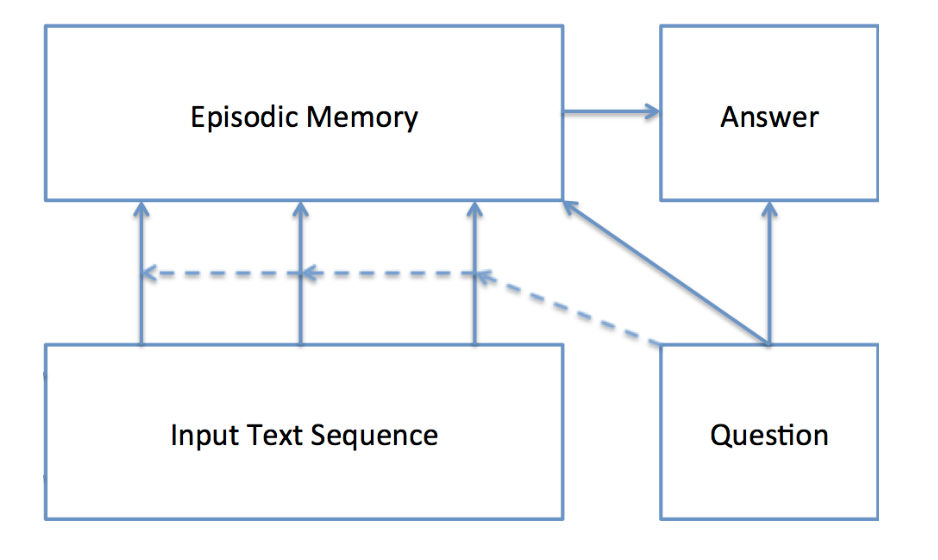
\includegraphics[width=0.6\textwidth]{./images/dynamic-memory-network-structure}
          \caption{Dynamic Memory Network模型架构}
      \end{figure} 
\subsubsection{输入模块}
输入模块接受一段文字,首先将文字中的每个单词转换为对应的词向量表示,然后将每个单词按顺序依次送入GRU。在每句话的结尾处,输出最终的隐式状态。
片段记忆模块将接收这些隐式状态,并进行总结推理。更加形式化的表示为,对于一个单词序列$T_I$ $w_1,...w_{T_I}$,我们根据下式来更新状态。\\
\begin{equation}
h_t = GRU(L[w_t],h_{t-1})
\end{equation}
然后对于由$T_I$作为子序列组成的序列$s_1,...s_{T_I}$,在每个子序列结束的时候,我们将最终的隐式状态$h_{s_1},...,h_{s_{T_I}}$输出
\subsubsection{问题模块}
问题模块与输入模块相似,接受问题作为输入,将问题序列中的每个单词转换为对应的词向量的表示,然后将每个词向量送入GRU,当所有问题单词都送入后,输出GRU的最终表示。
所以对于问题,形式化的表示为,对于一个包含单词$w_1,...,w_{T_Q}$的问题$T_Q$,我们使用下式更新隐式状态\\
\begin{equation}
h_t = GRU(L[w_t],h_{t-1})
\end{equation}
最后的输出为$h_{T_Q}$
\subsubsection{片段记忆模块}
片段记忆模块对于输入模块在每句话结束时输出的隐式状态和问题模块输出的隐式模块进行总结推理,产生一个最终记忆状态输出给回答模块,用于产生回答。\\
片段记忆模块主要由嵌套的两层GRU组成,内层GRU负责产生片段序列,外层GRU使用问题向量初始化后,根据片段序列产生最终记忆模块作为输入。\\
内层GRU每次通过遍历输入模块的输入序列产生一个片段,在每个片段结束后,内层GRU会把这个片段产生的最终状态送入外层GRU,下面的公式给出了内层GRU更新状态的方法:\cite{xiong2016dynamic}\\
\begin{equation}
z^i_t = [t_t,m,q,c_t \odot q, c_t \odot m,| c_t - q |,|c_t - m|]
\end{equation}
\begin{equation}
Z^i_t = W^{(2)}tanh(W^{(1)}z^i_t+b^{(1)})+b^{(2)}
\end{equation}
\begin{equation}
g^i_t = \frac{exp(Z^i_t)}{\sum_{k=1}^{M_i}exp(Z^i_k)}
\end{equation}
\begin{equation}
h^i_t = g^i_tGRU(c_t,h^i_{t-1} + (1 - g^i_t))h^i_{t-1}
\end{equation}
上面的式子中结合当前状态$c_t$,当前记忆状态$m$和记忆状态$q$来决定当前句子是否值得编码进入回答$g^i_t$中,如果$g^i_t \approx 0$,当前句子将被忽略,现在的状态即为之前的状态。
这个片段的最终状态是当内层GRU遍历晚所有句子之后产生的状态$e^i = h_{T_I}$\\
外层GRU将根据之前的记忆状态和本次片段状态来更新片段状态。\\
\begin{equation}
m^t = GRU(e^t,m^{t-1})
\end{equation}
外层GRU的最终记忆状态将被送入回答模块。
\begin{figure}[h]
      \centering
        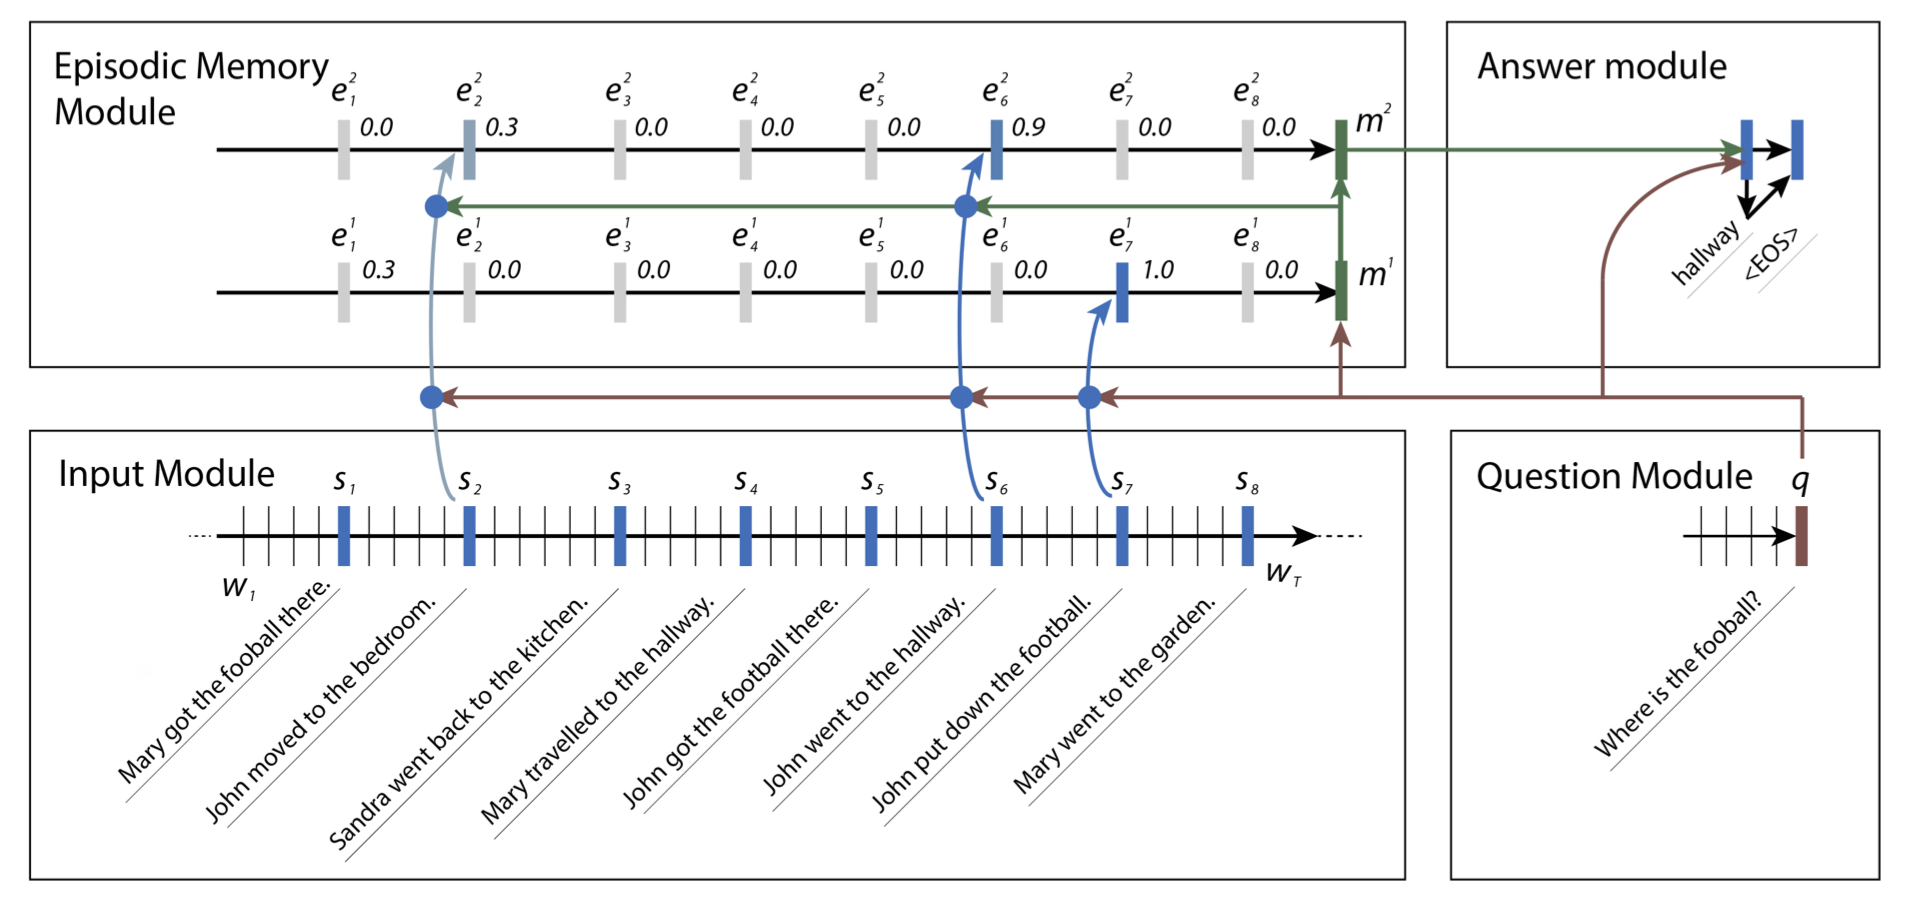
\includegraphics[width=0.9\textwidth]{./images/episodic-memory-structure}
          \caption{片段记忆模块架构}
      \end{figure}
\subsubsection{回答模块}
回答模块通过softmax产生对于回答标签的概率分布,然后产生单个单词回答,也可以将输入状态向量RNN来产生多个单词的回答。
\section{预期研究结果}
本次毕设预期结果是实现基础Dynamic Memory Network,对起进行优化,提高回答准确率,在单词回答的技术上支持多词回答,并且最终应用到技术文档中。
\section{进度计划}
\begin{itemize}
\item 3月31日$\sim$4月10日:编写基准模型和基础Dynamic Memory Network模型 
\item 4月11日$\sim$4月17日:训练、验证和测试基准模型和基础Dynamic Memory Network模型
\item 4月18日$\sim$4月25日:编写代码,尝试对Dynamic Memory Network进行优化
\item 4月26日$\sim$4月29日:编写中期报告
\item 4月30日$\sim$5月16日:尝试拓展Dynamic Memory Network,使模型具备多单词回答
\item 5月17日$\sim$5月29日:编写论文                       
\item 5月30日$\sim$答辩前:准备答辩 
\end{itemize}

{\sanhao\heiti\filcenter \centerline{本科毕业论文文献综述}}
\section{国内外发展现状}
早期的问答系统例如Baseball\cite{green1961baseball}是针对特定的知识领域所设计的可扩展性比较差,适用范围也比较小。随着互联网的发展,研究人员可用的语料信息的增加。
问答系统的发展得到了极大的提升,先后提出了基于逻辑推理的方法\cite{moldovan2001logic}、基于模版匹配的方法\cite{soubbotin2001patterns}、基于机器学习的方法\cite{yang2002integration}和基于数据冗余的方法\cite{kwok2001scaling}。
这些模型主要利用信息检索或浅层语义理解技术去从大量候选集中寻找答案从而构建智能问答系统,但是检索式问答技术存在一个缺陷,就是答案中一定至少包含一个用户问句中含有的字或者词,但是这在实际情况中往往是不成立的。在此阶段,阻碍问答系统进一步发展的主要困难是高质量的数据集和自然语言处理技术。
随着互联网的进一步发展,高质量的语料得到不断积累。而统计机器学习方法的兴起,自然语言处理技术各个子领域都取得了很大的进步,阻碍问答系统最大的两个问题正在逐步解决。正因如此,很多基于问答系统的产品也逐渐问世,例如:苹果的Siri、谷歌的Google Assistant和微软的Cortana。
\section{研究方向}
实现一个完整的问答系统主要需要三个部分,分别是用户问句的语义理解、信息检索和表示以及对知识进行推理,从而得到最终答案。
\subsection{问句理解}
这个环节实际上要解决的问题是如何将自然语言最准确地转化为计算机可以表示和理解的形式。主要有两种传统的方法来实现,分别是语义解析的方法和基于信息检索的方法。\\
基于语义解析的方法中目前最主流的是组合范畴语法 CCG\cite{kwiatkowski2011lexical}\cite{zettlemoyer2012learning}。CCG首先自然语言问句中的词汇被映射到语义表达式中的词汇,然后按照特定的语法规则将词汇组合起来,进而得到了最终的语义表达式。\\
基于信息检索的方法,首先使用分词、实体识别等NLP技术找到问句中所涉及到的实体和关键词,然后去知识资源库中去进行检索。
\subsection{知识图谱的构建}
知识图谱的构建,主要是将互联网上存在的大量非结构化的文字语料,结构化,并且存储到知识数据库中。在这个过程中,我们需要先对文本进行实体识别,然后对实体进行分类和消歧,接着抽取出关系和事件,这样就能构建一个由实体、关系和事件组成的知识数据库。
目前代表性的工作有:TextRunner\cite{yates2007textrunner}、Wanderlust\cite{akbik2009wanderlust}、NELL\cite{kwiatkowski2011lexical}等。
\subsection{知识推理}
早期的知识推理方法大多对现有知识归纳学习出符号逻辑的推理规则,比如PRA\cite{lao2011random}.这种方法随着推理规则的数量随着关系的数量指数增长,因此很难扩展到大规模知识图谱中去。而随着神经网络等发展,基于Memory和Attention机制等神经网络,在知识归纳推理方面取得了令人瞩目的结果。
这也是我这次毕设的研究基础。\\
\section{关键技术}
\subsection{Word2Vec}
Word2Vec(Mikolov et al., 2013\cite{mikolov2013efficient})是一种表达词汇的方法,将一个单词用一个向量来表示,关系比较近的词(例如:king和queen,Shanghai和Beijing)在向量空间相对应的有比较近的距离。如何确定词的关系,一个朴素的想法就是在相似上下文中出现的单词关系比较近。
Word2Vec就是基于这一想法的一种高效的词汇表达方法。特别的,Word2Vec有两种算法,分别是Continuous Bag-of-Words(CBOW)和Skip-Gram。CBOW是根据环境词预测中心词,而Skip-Gram是根据中心词预测环境词。\\
\subsection{GloVe}
尽管Word2Vec已经被实验证明可以发掘出复杂的语义相似关系,但是是根据局部上下文来预测,往往忽略了整体的信息。与之对应的,Pennington et al.\cite{pennington2014glove}提出的Global Vectors for Word Representation (GloVe)使用全局的统计信息预测单词$i$出现在单词$j$的上下文中的概率。
具体来讲,GloVe使用最小二乘作为目标函数训练词词共生矩阵。GloVe在很多词汇相似性任务中已经表现出优越的结果。\\
\subsection{递归神经网络(RNN)}
递归神经网络是一种特别适合对时序信息建模的神经网络架构。在$t$时刻,RNN输入词矩阵$w_t$和上一步的隐式状态向量$h_{t-1}$进行下面的运算后,产生这一步点隐式状态向量:\\
\begin{equation}
h_t = f(Wx_t+Uh{t-1}+b)
\end{equation}
上式中$W$,$U$和$b$是这个RNN的参数。使用RNN对语段建模,能够提取到当前词的前面的所有词的信息考虑在内。
\subsection{GRU}
尽管RNN能够考虑时序关联信息,但是由于使用backpropagation进行优化目标函数时,求导产生的链式相乘,会导致,随着递归向前,产生权重指数级爆炸或消失的问题,难以捕捉长期时间关联。对于权重指数暴炸问题,可以简单的采用超出阈值后截断的方法,就能产生很好的结果。
而Chung et al.\cite{chung2015gated}Gated Recurrent Units(GRU)是一种激活单元,就是为了解决权重指数消失问题,对网络结构进行的优化。下面的一组公式表明了GRU如何根据$h_{t-1}$和$x_t$产生$h_{t}$:\\
\begin{equation}
z_t = \sigma (W^{(z)}x_i + U^{(z)}h_{t-1})
\end{equation}
\begin{equation}
r_t = \sigma (W^{(r)}x_i + U^{(r)}h_{t-1})
\end{equation}
\begin{equation}
\widetilde{h}_t = tanh(r_t \odot Uh_{t-1} + Wx_t)
\end{equation}
\begin{equation}
h_t = (1-z_t) \odot \widetilde{h}_t + z_t \odot h_{t-1}
\end{equation}
式(2)确定了$h_{t-1}$应该多大程度被带入下一阶段。式(3)表明$h_{t-1}$多大程度上影响$\widetilde{h}_t$。式(4)表明新的记忆$\widetilde{h}_t$是由输入$x_t$和$h_{t-1}$确定的。
式(5)表明隐式状态$h_t$最终是由以前的隐式状态$h_{t-1}$和$\widetilde{h}_t$新的记忆组成的。
\subsection{LSTM}
Long Short Term Memories(LSTM)\cite{hochreiter1997long}是另一种与GRU相似的激活单元,与GRU起到的作用相同。下面一组式子表明了LSTM的数学结构:\\
\begin{equation}
i_t = \sigma (W^{(i)}x_t + U^{(i)}h_{t-1})
\end{equation}
\begin{equation}
f_t = \sigma (W^{(f)}x_t + U^{(f)}h_{t-1})
\end{equation}
\begin{equation}
o_t = \sigma (W^{(o)}x_t + U^{(o)}h_{t-1})
\end{equation}
\begin{equation}
\widetilde{c}_t = tanh(W^{(c)}x_t + U^{(c)}h_{t-1})
\end{equation}
\begin{equation}
c_t = f_t \odot c_{t-1} + i_t \odot \widetilde{c}_t
\end{equation}
\begin{equation}
h_t = o_t \odot tanh(c_t)
\end{equation}
式(6)使用输入词和之前的隐式状态来判断输入词是否值得保存,用来产生新记忆。式(7)用来评估过去的记忆是否对于计算现在的记忆有用。
式(8)确定了最终记忆应该多大程度上保存到隐式状态中。式(9)根据输入词$x_t$和$h_{t-1}$产生新的记忆。式(10)根据新记忆和$h_{t-1}$产生最终记忆。
\subsection{Attention机制}
一句话中的不同的单词的重要性是不同的,例如名词、动词在就会比定冠词介词表达更多的意思。Bahdanau et al\cite{Bahdanauetal.2014}注意到了使用单向量的RNN的最终状态没有办法很好的表征不同输入的部分有不同重要性这一特征。
更近一步的,输出的不同部分可能更看重输入的特定部分。例如,在翻译中,输出的前几个单词通常是根据输入的前几个单词,而输出的后几个单词则更多的依赖于输入的后几个单词。\\
针对这一特点,Attention机制在编码的每一步,首先观察整个输入序列,然后决定在这一个阶段,哪一部分比较重要。\\
Bahdanau et al.提出的模型主要分成两个部分,编码部分和解码部分。编码部分对输入序列编码为向量,解码部分提取编码信息解码成语句,输出语句有一系列单词组成$y_1,...,y_m$。
\subsubsection{编码器}
令$(h_1,...,h_n)$为每个输入句子的隐式向量,这些向量可以使用GRU或者LSTM来产生,包含了词在上下文中的表达信息。
\subsubsection{解码器}
我们可以通过下面的递归式计算隐式状态$s_i$
\begin{equation}
s_i = f(s_{i-1},y_{i_1},c_i)
\end{equation}
在这里$s_{i-1}$是前一个隐式状态,$y_1$是上一个输出单词,上下文向量$c_i$是在解码的第$i$步根据解码状态对原文全文信息等提取表示。\\
对于输入序列中的隐式向量,计算下式得到一个权重值
\begin{equation}
e_{i,j} = a(s_{i-1},h_j)
\end{equation}
上式中$a$可以是任何定义域是$R$的函数,上市会得到一系列值$e_{i,1},...,e_{i,n}$。使用softmax归一化
\begin{equation}
\alpha_{i,j} = \frac{exp(e_{i,j})}{\sum_{k=1}^nexp(e_{i,k})}
\end{equation}
最后对输入隐式序列加权后生成最终的上下文状态向量。
\begin{equation}
c_i = \sum_{j=1}{n}\alpha_{i,j}h_j
\end{equation}
直观的来讲,这个向量能够在第$i$步捕获原文的上下文信息。
\subsection{Dynamic Memory Network}
Kumar et al.\cite{DBLP:journals/corr/KumarISBEPOGS15} Dynamic Memory Network由四个模块组成,分别是:输入模块、片段记忆模块、问题模块、回答模块。整体的架构如图表所示。\\
\begin{figure}[h]
      \centering
        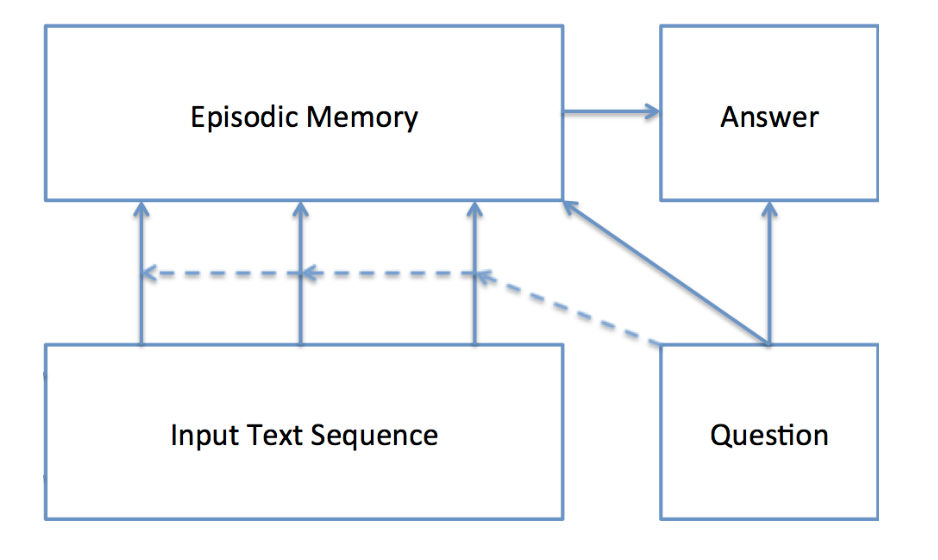
\includegraphics[width=0.6\textwidth]{./images/dynamic-memory-network-structure}
          \caption{Dynamic Memory Network模型架构}
      \end{figure} 
\subsubsection{输入模块}
输入模块接受一段文字,首先将文字中的每个单词转换为对应的词向量表示,然后将每个单词按顺序依次送入GRU。在每句话的结尾处,输出最终的隐式状态。
片段记忆模块将接收这些隐式状态,并进行总结推理。更加形式化的表示为,对于一个单词序列$T_I$ $w_1,...w_{T_I}$,我们根据下式来更新状态。\\
\begin{equation}
h_t = GRU(L[w_t],h_{t-1})
\end{equation}
然后对于由$T_I$作为子序列组成的序列$s_1,...s_{T_I}$,在每个子序列结束的时候,我们将最终的隐式状态$h_{s_1},...,h_{s_{T_I}}$输出
\subsubsection{问题模块}
问题模块与输入模块相似,接受问题作为输入,将问题序列中的每个单词转换为对应的词向量的表示,然后将每个词向量送入GRU,当所有问题单词都送入后,输出GRU的最终表示。
所以对于问题,形式化的表示为,对于一个包含单词$w_1,...,w_{T_Q}$的问题$T_Q$,我们使用下式更新隐式状态\\
\begin{equation}
h_t = GRU(L[w_t],h_{t-1})
\end{equation}
最后的输出为$h_{T_Q}$
\subsubsection{片段记忆模块}
片段记忆模块对于输入模块在每句话结束时输出的隐式状态和问题模块输出的隐式模块进行总结推理,产生一个最终记忆状态输出给回答模块,用于产生回答。\\
片段记忆模块主要由嵌套的两层GRU组成,内层GRU负责产生片段序列,外层GRU使用问题向量初始化后,根据片段序列产生最终记忆模块作为输入。\\
内层GRU每次通过遍历输入模块的输入序列产生一个片段,在每个片段结束后,内层GRU会把这个片段产生的最终状态送入外层GRU,下面的公式给出了内层GRU更新状态的方法:\cite{xiong2016dynamic}\\
\begin{equation}
z^i_t = [t_t,m,q,c_t \odot q, c_t \odot m,| c_t - q |,|c_t - m|]
\end{equation}
\begin{equation}
Z^i_t = W^{(2)}tanh(W^{(1)}z^i_t+b^{(1)})+b^{(2)}
\end{equation}
\begin{equation}
g^i_t = \frac{exp(Z^i_t)}{\sum_{k=1}^{M_i}exp(Z^i_k)}
\end{equation}
\begin{equation}
h^i_t = g^i_tGRU(c_t,h^i_{t-1} + (1 - g^i_t))h^i_{t-1}
\end{equation}
上面的式子中结合当前状态$c_t$,当前记忆状态$m$和记忆状态$q$来决定当前句子是否值得编码进入回答$g^i_t$中,如果$g^i_t \approx 0$,当前句子将被忽略,现在的状态即为之前的状态。
这个片段的最终状态是当内层GRU遍历晚所有句子之后产生的状态$e^i = h_{T_I}$\\
外层GRU将根据之前的记忆状态和本次片段状态来更新片段状态。\\
\begin{equation}
m^t = GRU(e^t,m^{t-1})
\end{equation}
外层GRU的最终记忆状态将被送入回答模块。
\begin{figure}[h]
      \centering
        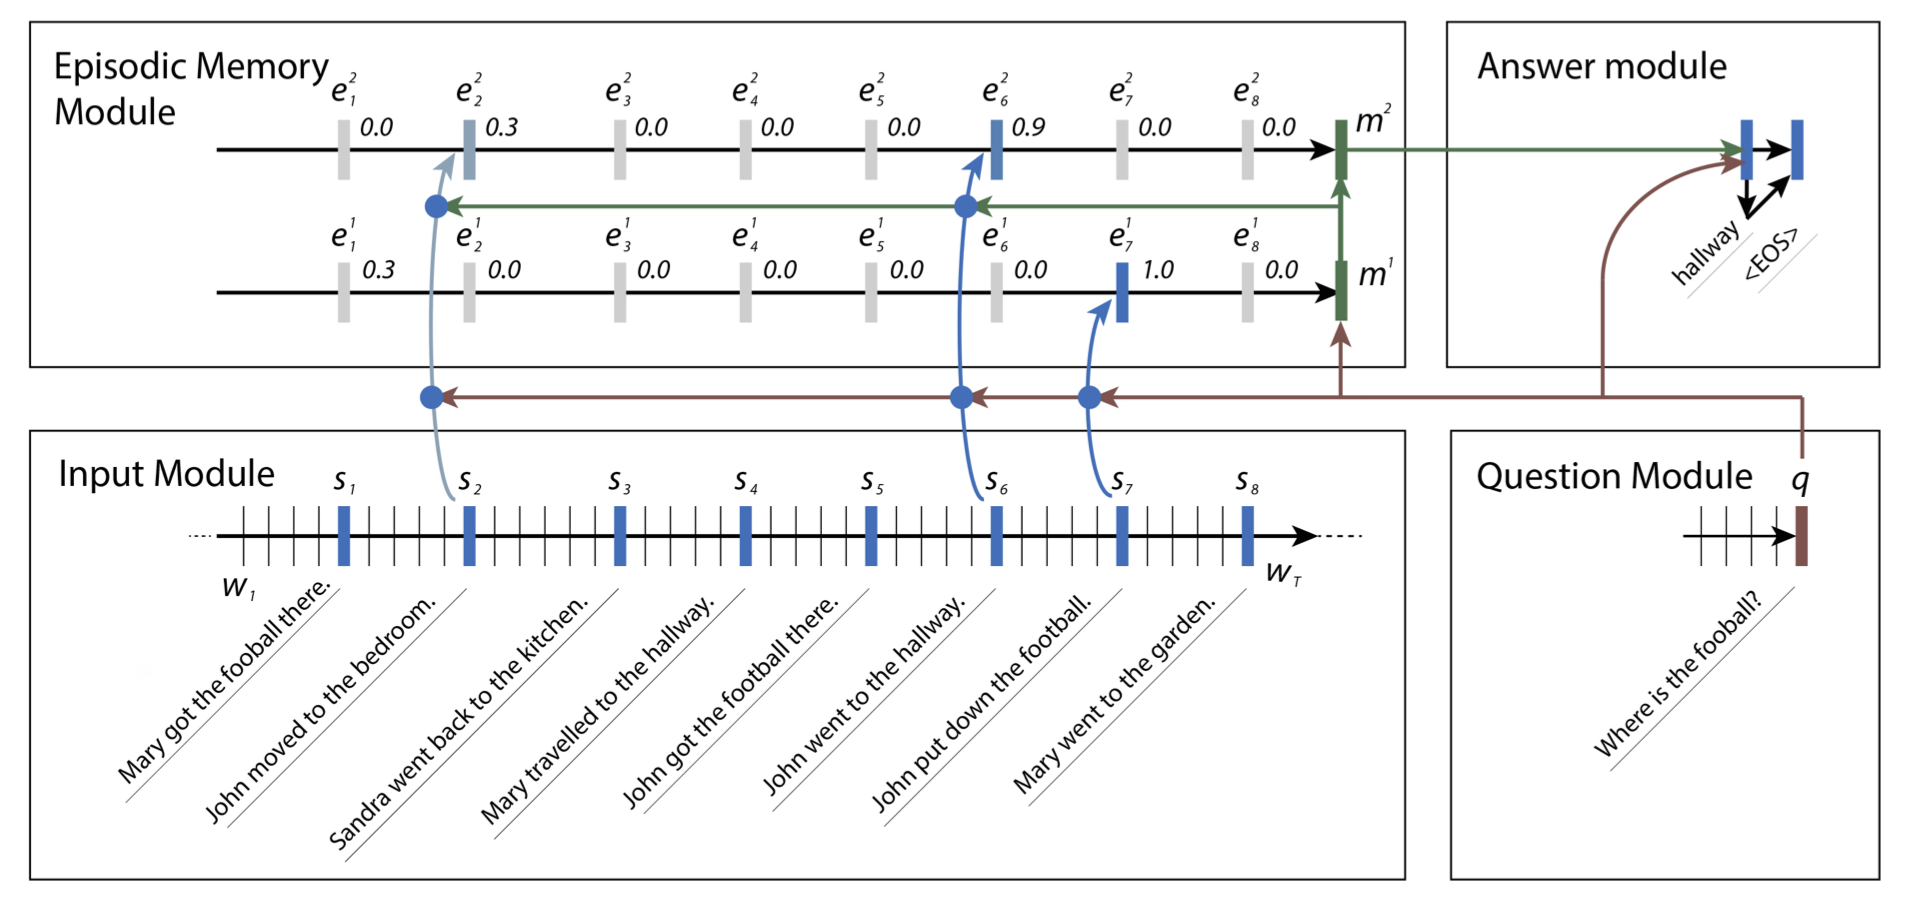
\includegraphics[width=0.9\textwidth]{./images/episodic-memory-structure}
          \caption{片段记忆模块架构}
      \end{figure}
\subsubsection{回答模块}
回答模块通过softmax产生对于回答标签的概率分布,然后产生单个单词回答,也可以将输入状态向量RNN来产生多个单词的回答。
%     \bibliography{data/zjubib}
%   %\chapter{本科毕业论文外文翻译}
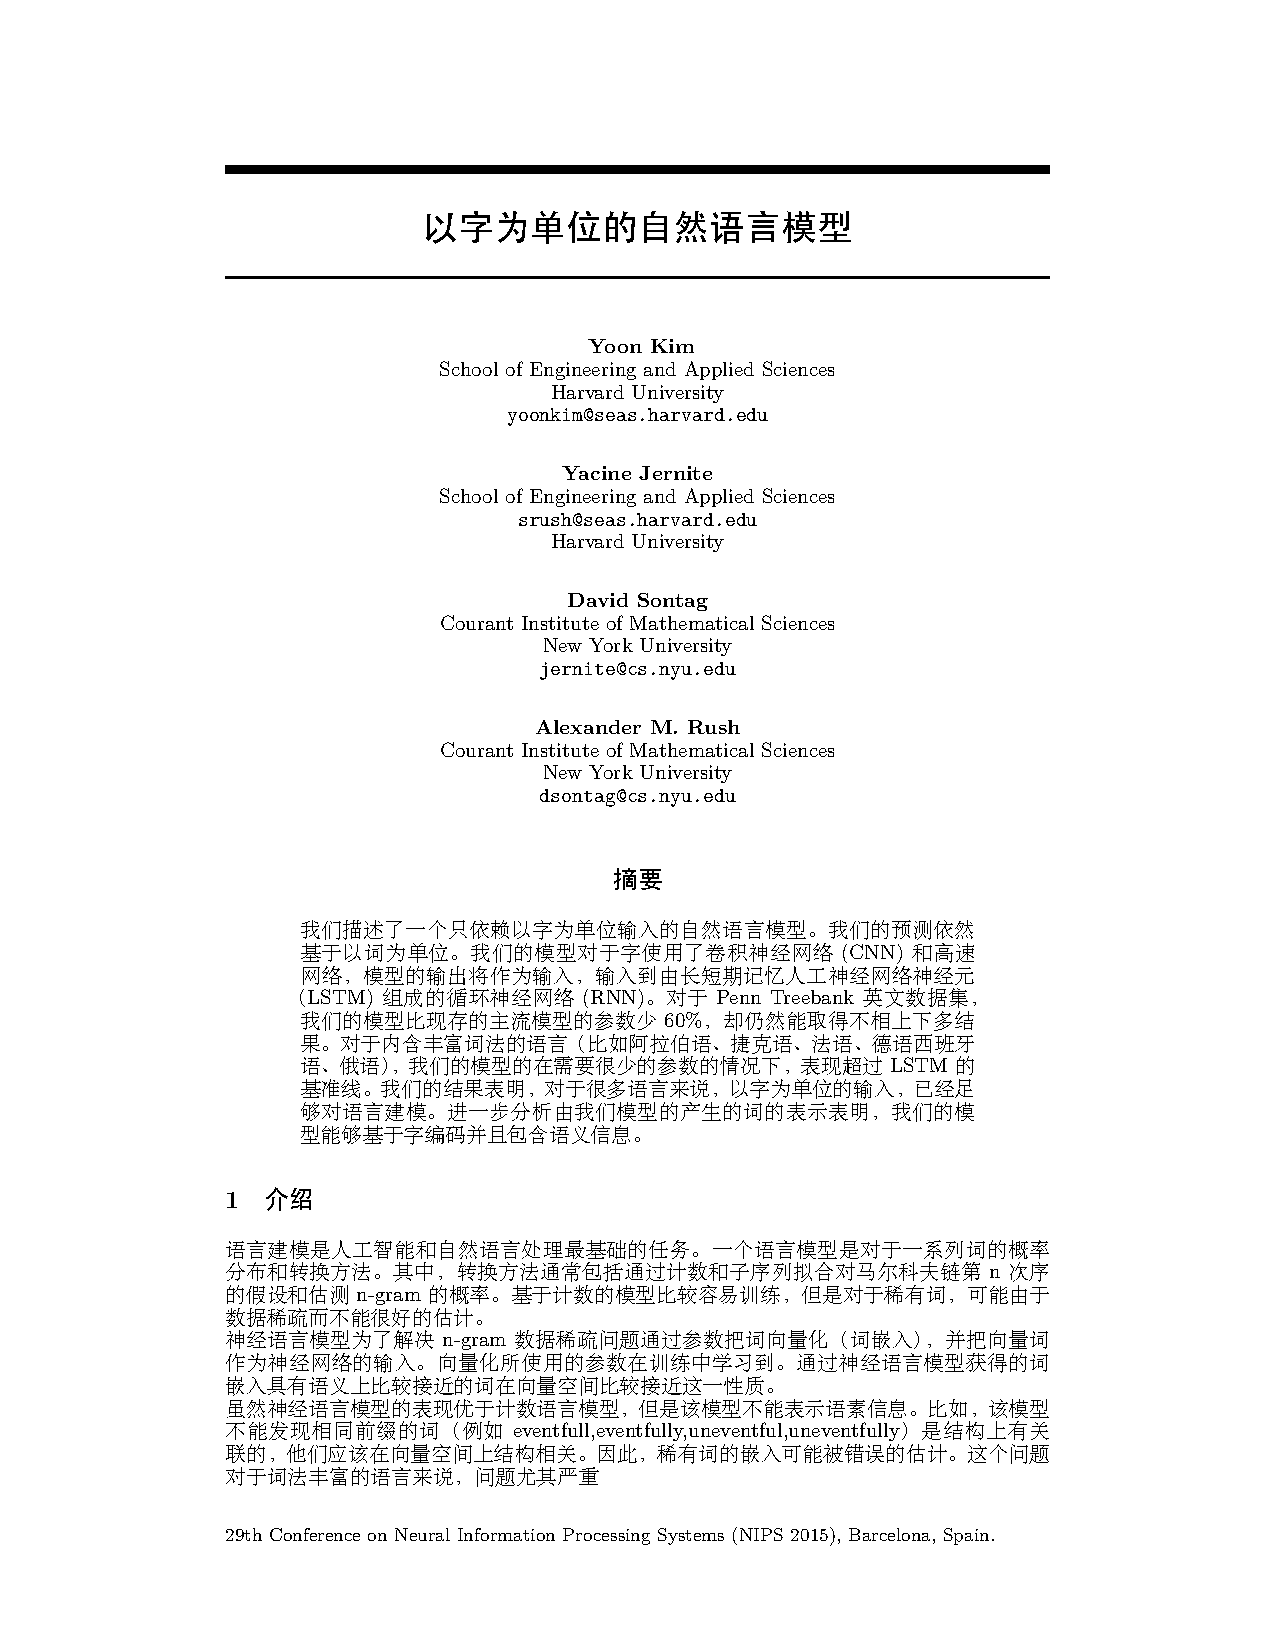
\includepdf[pages=-]{./data/translate-paper-chinese.pdf}
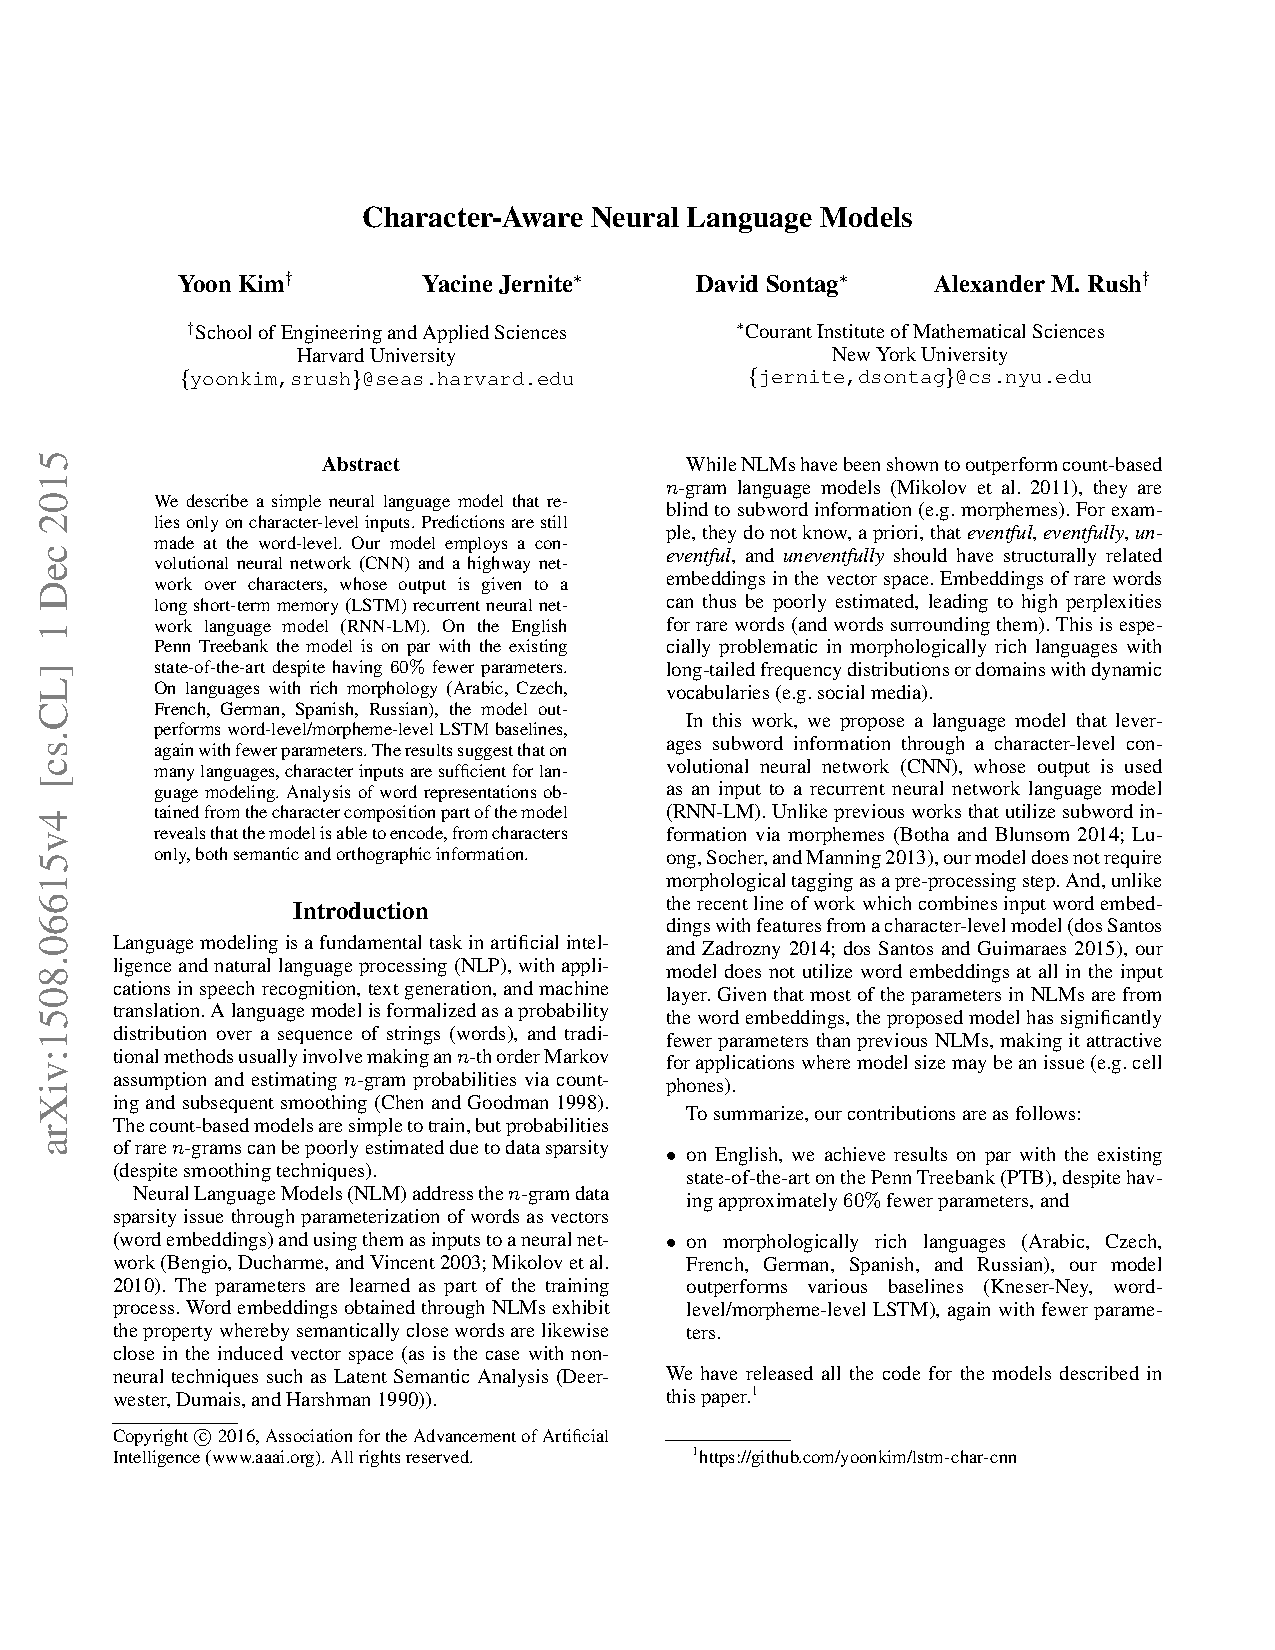
\includepdf[pages=-]{./data/translate-paper-english.pdf}
% %==============================================================
% %这也是个不需要自己修改的部分。

%   \backmatter %结束章节自动编号

%==============================================================
\end{document}
